\documentclass[letterpaper,11.5pt]{scrartcl}
\usepackage{totcount}
% \documentclass[11pt]{report}
% \documentclass{report}
% \documentclass{book}
\usepackage[bookmarks, hidelinks]{hyperref}
\usepackage{amssymb,amsmath}
\usepackage[title]{appendix}
% \usepackage{fullpage}
\usepackage{tabulary}
\usepackage{tabularx}
\usepackage{float}
% \usepackage[margin=0.50in]{geometry}
\usepackage[margin=1.00in]{geometry}

\usepackage{booktabs}
\usepackage{pslatex}
\usepackage{apacite}
\usepackage{caption}
% \usepackage{subcaption}
\usepackage{wrapfig}
\usepackage[english]{babel}
\usepackage{lmodern}
\usepackage{setspace}
\doublespace
% \usepackage{url}
\usepackage{bigfoot}
\usepackage[export]{adjustbox}
\setlength\intextsep{0pt}

% Colored comments 
\usepackage{color}
\definecolor{myorange}{RGB}{240, 96, 0}
\newcommand{\mt}[1]{{\textcolor{myorange} {({\tiny MT:} #1)}}}

\definecolor{myblue}{RGB}{30,144,255}
\newcommand{\jhj}[1]{{\textcolor{myblue} {({\tiny JHJ:} #1)}}}

\definecolor{mypurple}{RGB}{148,0,211}
\newcommand{\cm}[1]{{\textcolor{mypurple} {({\tiny CM:} #1)}}}

\definecolor{mygreen}{RGB}{26, 153, 51}
\newcommand{\ps}[1]{{\textcolor{mygreen} {({\tiny PS:} #1)}}}

\newtotcounter{citnum} %From the package documentation
\def\oldbibitem{} \let\oldbibitem=\bibitem
\def\bibitem{\stepcounter{citnum}\oldbibitem}

\usepackage{graphicx}


%\title{The form of uncertainty affects selection for social learning}
\title{Different forms of uncertainty differently affect the evolution of social learning}

\author{{}}

\begin{document}
\maketitle

\newcommand{\pisub}[1]{\pi_{\mathrm{#1}}}
\newcommand{\pilow}{\pisub{low}}
\newcommand{\pihigh}{\pisub{high}}
\newcommand{\piI}{\langle \pisub{I} \rangle}
\newcommand{\piS}{\langle \pisub{S} \rangle}
\newcommand{\ledger}{\bar\pi_{ib}}

\newcommand{\meanvar}[1]{\langle #1 \rangle}
\newcommand{\meansl}{\meanvar{s}}
\newcommand{\meanpi}{\meanvar{\pi}}
\newcommand{\meansoc}{\meanvar{\pi_\mathrm{S}}}
\newcommand{\meanasoc}{\meanvar{\pi_\mathrm{A}}}
\newcommand{\meanT}{\meanvar{T}}

\newcommand{\bandit}{\text{Bandit}_b(0, 1)}

\begin{abstract}

Social learning is essential to human survival. It is likely to evolve when it is more
efficient than asocial, trial-and-error learning. Theoretically, social learning
is adaptive for some uncertainty, but too much uncertainty makes
social information unreliable. This fact is empirically
supported across biology and human sciences. However, it is unclear how
specific classes and types of uncertainty affect social
learning evolution. Furthermore, existing models and experimental operationalizations of
uncertainty are ambiguously related, and 
tend to only consider a small number of behavioral
choices.  Here we use evolutionary agent-based modeling to consolidate
models of uncertainty in social learning evolution to address these issues.
We model societies of agents who perform one of a number
of possible behaviors to acquire payoffs in a time-varying environment.
We identified complex patterns in social learning evolution depending on contextual
uncertainty variables: environmental variability, ambiguous payoffs, 
decision sets size, and effective lifespans. 
Our work advances social learning evolution theory in a way that could help 
guide human, non-human, and artificial intelligence towards optimal responses 
to existential threats and new opportunities.\footnote{This document contains
\total{citnum} references.}  
\end{abstract}


\section{Introduction}
\cm{Notes on our June 2 discussion (USPs): "Uncertainty favors social learning" is a widespread belief. But it is operationalized in different ways, and oftentimes it does not reflect REAL uncertainty. Selling points of this paper 1) real uncertainty, 2) 4 kinds uncertainty, 3) cognition (soft-max temperature varies how much explores).}


%% for inclusion in the social learning ms

Decision-making under uncertainty is fundamental challenge for any organism. Uncertainty weighs particularly heavily on humans adaptation because of our long lifespans, cosmopolitan distribution, and the resulting necessity to adapt to relatively coarse-grain environments \cite{levins1962}.

While the importance of decision-making under uncertainty is generally acknowledged, there is often some confusion about what constitutes uncertainty. First, uncertainty needs to be distinguished from risk. While the concepts sound similar, uncertainty and risk are quite different. Both refer to the existence of non-deterministic outcomes, but with risk, outcomes can be represented probabilistically, whereas uncertainty implies that the probabilities of outcomes remain unknown \cite{knight1921}. As it doesn't lend itself to simple mathematical representation, uncertainty presents substantial analytical challenges as first noted by \cite{keynes1921}.

Despite the technical difficulties of dealing with uncertainty, addressing it is an essential task because it potentially changes our understanding of decision-making in a qualitative manner. The dominant approach to understanding decisions for choices with variable outcomes is expected utility theory (EUT). As the name suggests, EUT requires the ability to calculate expectations, which means that we must know the probability distributions of outcomes. The non-probabilistic nature of uncertainty means one cannot calculate expectations. Following \cite{savage1954}, various research traditions in decision theory and economics have treated uncertainty as if it were risk, just with subjective probabilities replacing objective ones. The fundamental problem with this approach was noted by \cite{geweke2001} and further developed by \cite{weitzman2009}. In particular, the probability density function of an outcome that needs to be learned, but for which opportunities for learning are highly constrained, will be heavy-tailed and expected-utility calculations will not work because of the resulting undefined mass-generating function. Uncertainty implies heavy-tailed probability distributions and heavy-tailed distributions require different analytical methods \cite{nair_etal2022}.

The heuristic-based adaptive-toolbox approach of \cite{todd_gigerenzer2000} provides an alternative strategy for understanding decision-making under uncertainty. There is a strong intuition that uncertainty should activate specific social-learning heuristics. Within the cultural-evolution literature, uncertainty is generally thought to lead to a social heuristic known as \emph{conformist-biased learning} \cite{boyd_richerson1985, henrich_boyd1998, muthukrishna_etal2016}.

True uncertainty arises when an organism lacks the capacity to learn about the possible outcomes of a decision task. This is very likely for a cosmopolitan species living in a coarse-grain environment. Task complexity also. Non-stationary environmental change \cite{kay_king2020}. These potential sources of uncertainty can also interact. 


\cm{CUT in favor of uncertainty intro: Social learning enhances problem solving when acquiring information from others is more efficient than learning on one's own~\cite{Laland2004}. However, social learning can also lead individuals astray if, for example, they are copying outdated information. Theoretical models have helped clarify the circumstances under which social learning should be evolutionarily favored. For example, environments that change across time favor learning from others (as opposed to having a genetically fixed behavior) ~\cite{BoydRicherson1985,Henrich1998}, so long as the environments are not so variable that the social information reflects outdated and maladaptive behavior point~\cite{Rogers1988,Feldman1996, aoki2014evolution}. \cm{check that the citations still accurate}. This theoretical work has motivated much empirical research and helped predict social learning behavior in humans and other species ~\cite{McElreath2005,Kendal2018,Allen2019}.
}

From this literature, the idea that uncertainty supports social learning has proliferated, but the term ``uncertainty" often conflates several different interpretations of that word. For example, different models define uncertainty in terms of the rate of environmental change, the correlation between spatial environments, or the reliability of information acquired from the environment. 
Furthermore, in translating mathematical models to verbal predictions, the formal meaning of terms like uncertainty is often lost \cite{lawson1988probability}, facilitating such conflation. 
%Furthermore, a
And as the number of formal models of social learning have expanded, an ever increasing number
of modeling choices ~\cite[Figure 1]{Kendal2018} and formalizations of uncertainty have made it difficult to compare across models and consolidate our understanding of the contexts in which social learning is adaptive.  

To address these concerns we developed an empirically-motivated, evolutionary agent-based model that simultaneously operationalizes four %principal components 
different forms of uncertainty: (1) temporal environmental variability; (2) selection set size (the number of possible behaviors); (3) payoff ambiguity (the difference in the expected rewards for different behaviors); and (4) the effective lifespan of agents (the number of opportunities for individual learning). These were chosen because modeling and empirical 
studies across taxa tend use one or more of these uncertainty dimensions\ps{citation needed}.  
The model also involves a more cognitively realistic learning mechanism, the softmax algorithm, which allows us to more accurately assess some of the likely tradeoffs between social and individual learning. We use this integrated model to ask what kinds of uncertainty are likely to favor social learning, and to clarify the logic of why this would be the case. Answering this question is critical for understanding human behavior adapting to a rapidly changing world, both to mitigate existential threats~\cite{Moya2020,Jones2021}, and to capitalize on new opportunities such as transitioning to clean energy use and production~\cite{NatureEnergyEditorialPromisesPremises2018,Brisbois2022}.

In the remainder of this introduction, we further unpack our motivation for this work justify our approach. We then present our model and the results of our analyses. We conclude with a discussion of our results and their implications for our understanding of social learning, uncertainty, and cultural evolution. 

% \cm{I moved this for now: \emph{"Furthermore, many models of social learning evolution do not account for individual-level cognition~\cite{Heyes2016}, though humans clearly have evolved cognitive mechanisms for dealing with uncertainty generally~\cite{Gershman2019,Schulz2019}."} because I think it interrupted the flow and didn't seem directly linked to the goal of understanding aspects of uncertainty. However, if this is one of the main features of the model that we want to highlight as an improvement over previous work, then we probably have to say something more about it. Perhaps I just wasn't seeing the connection though, and the more accurate cognitive model DOES add to our ability to study the consequences of uncertainty. If that's the case, the argument should be sharpened. If not, maybe we put this info when the cognitive model is introduced.}\mt{Agreed. I put a first draft of a better version of this paragraph closer to/at the end of the Intro.}



%\mt{This paragraph is a first try to introduce the four uncertainty dimensions with examples to illustrate the problem we are answering. I outlined the next paragraph to get into more details of social learning: how cultural evolution works; conformity, success-biased, etc. Cristina, please edit this.} 

\subsection{Varieties of Uncertainty}

Uncertainty involves a reduced ability to predict what will happen in the future or to assess which actions are likely to yield particular outcomes. Uncertainty can manifest in many ways. We focus on the following four sources of uncertainty for the evolution of social learning: (1) temporal environmental variability, (2) selection set size, (3) payoff ambiguity, and (4) effective lifespan.

\textbf{Temporal environmental variability.}
When external or internal shocks (e.g., climatic events, migration, technological paradigm shifts) occur, strategies that were previously adaptive may no longer be optimal. The difficulty in predicting either when such shocks will occur or what behaviors will adaptive in the resulting environments leads to uncertainty. 
Temporal environmental variability is fundamental to most evolutionary models of social learning, yet even this is implemented in several ways. It is usually modeled as an independent probability of the environment changing its state each generation ~\cite{BoydRicherson1985,Rogers1988,Feldman1996,McElreath2005,Enquist2007,perreault2012bayesian,aoki2014evolution}. The probabilities of environmental change are usually fixed, %~\cite{BoydRicherson1985,Rogers1988,kendal2009evolution}, 
but they have also been modeled as deterministic cycles ~\cite{Feldman1996, aoki2014evolution} or as variable rates \cm{who does this?}\ps{Yeah, I'm not even sure what variable rates means in this context}. Furthermore, the consequences of environmental change can range from mild to  catastrophic. In the latter case, a change of environment results in the total elimination of any adaptive behavior, which must be learned \emph{de novo} for the new environment ~\cite{Rogers1988}. Such catastrophic environmental changes present a large adaptive challenge as individuals cannot bank on accumulated information from previous generations. Other models of environmental change introduce less uncertainty as they fluctuate between two environmental states with corresponding adaptive behaviors. This means that all individuals with previously maladaptive behaviors then have adaptive behaviors upon the environment changing ~\cite{perreault2012bayesian}. 

\textbf{Selection set size.}
When one does not know which option to take, uncertainty increases with the number of options. This is a mathematical fact at the core of information theory: the number of bits required to reliably encode the optimal solution increases by one every time the selection set doubles in size  \cite{mackay2003information}. 
This is intuitive; the more options one could potentially investigate, the greater one's uncertainty about which option is the best choice. In studies of social learning, the size of the selection set is very often limited to just two options. 
For example, in empirical studies of \emph{bombus terresteris} (bumble
bee)~\cite{Baracchi2018} and \emph{parus major} (great tit)~\cite{Aplin2017},
experimenters provided two behaviors for
the bees or birds to choose from, where one yielded a higher payoff than the other. %respectively, each yielding greater or smaller payoffs depending on experimental treatment. 
Many human studies have also used just two
or three possible behaviors~\cite{McElreath2005,Toyokawa2019}.
Modeling studies have often used just two 
behaviors~\cite{Rogers1988,Feldman1996,Rendell2010,perreault2012bayesian}, though others have studied systems with larger selection sets where the number of options is usually not explicitly specified~\cite{boyd1995does,Enquist2007}. It is very rare, however, to find the size of the selection set manipulated as a measure of changing uncertainty. 

\textbf{Payoff ambiguity.}
Many models of social learning differentiate between the payoffs for adopting optimal vs. non-optimal behaviors \cite{Rogers1988,Enquist2007,Rendell2010}. The size of the difference between these payoffs is usually taken to indicate the strength of selection of learning, which makes sense. However, in reality payoffs for particular behaviors are not always consistent. A behavior may yield a large payoff sometimes and a small payoff other times \cite{McElreath2005}. This means that signals about the relationship between behavior and payoff are often noisy, and differentiating between behavioral options is in part a problem of signal detection.
When the difference in expected payoffs between optimal and non-optimal behaviors is very large, this noise matters little, as the signal is still very clear. However, when the expected payoffs of different behaviors are similar relative to the size of their variances, ambiguity arises about which behaviors really are superior. Smaller differences between payoffs corresponds to larger ambiguity.    
Importantly, payoff ambiguity %differs from selection set size in that it not only affects uncertainty, it also directly
influences both uncertainty \emph{and} the strength of selection. %This parameter sometimes takes the form of differences in expected payoffs arising from different behaviors or strategies~\cite{Enquist2007,Rendell2010} or by varying the standard deviation of payoffs~\cite{McElreath2005}. 

\textbf{Effective lifespan.}
Learning can be viewed as a process by which an individual reduces or otherwise manages their uncertainty \cite{jacobs2011bayesian,clark2013whatever}. It is an iterative process by which one repeatedly acquires information, forms representations and predictions, and tests and refines those representations and predictions. It therefore stands to reason that the more opportunities one has for learning, the more one can in principle reduce one's uncertainty. Similarly, a reduction in the number of opportunities to learn will increase the uncertainty about whether one has accurately learned about the available behavioral options and their associated payoffs. We refer to the number of learning opportunities as an individual's effective lifespan to imply that it is the number of opportunities to learn throughout the individual's lifespan that matters here, not necessarily how long they live in the absence of relevant learning opportunities. Empirically, the age of an individual will often correspond with the number of learning opportunities they have had.  Aplin et al. (2017) \nocite{Aplin2017} found that younger great tits more readily used social information compared with older individuals, possibly because they had  accrued less information via individual learning, and also possibly because younger individuals have the most to gain (given their expected remaining lifespan) by switching to superior behavioral options. \ps{I got rid of the Leris and Reader reference because it didn't seem relevant to age-based uncertainty. They just showed that young guppies exposed to reliable models were more likely to use social information later. I also added some human studies, which seems important.} Cross-cultural studies on humans have shown that young children are more likely to acquire their beliefs and simple skills from their parents than are older children or adults, which is also at least partly due to the differential knowledge accrual between young children and the older adults to whom they direct the most trust and attention \cite{kline2013teaching, Reyes2016}. \cm{not sure the second phrase is warranted. Can't seem to find whether social learning overall is  }
%The age of individuals was found to have an effect on social learning in both \emph{parus major}~\cite{Aplin2017} and \emph{poecilia reticulata} (guppies)~\cite{Leris2016}. \ps{What effect? I'm not sure }
%\mt{Need better connection between lifespan and age, or better references to support use of lifespan}.
Individuals with shorter effective lifespans will end their lives with more uncertainty about which behaviors are optimal, and thereby transmit some of that uncertainty to anyone who learns from them. The effective lifespan for learning varies both across individuals and across species, yet there is little formal theory incorporating this form of uncertainty into our understanding of the evolution of social learning. 

%To answer our research questions about the combined effect of various forms of uncertainty on social learning evolution, we developed an agent-based model that incorporates all four of these uncertainty variables. We systematically vary these parameters to understand and predict their effects on social learning evolution.

\subsection{Varieties of learning, social and otherwise} (CRISTINA) 
\cm{I think a lot of this may be too much detail. I'm still editing and focusing the above on the main forms of uncertainty we are modeling and reviewing the relevant literature as we go. Yes we've made choices about things like horizontal vs vertical, but i think we can just justify that when we introduce the model }
\ps{I agree with Cristina here. I think we should use this section to justify our way of modeling individual and social learning, which is different from previous models. We don't need to provide a detailed review, just why it's worth doing it as we've done it. In particular, we should set up (1) social learning as an initial scaffold for future social learning, and (2) softmax individual learning which involves some greediness with occasional trial and error.}
To add to confusion about how to integrate diverse models of social learning
evolution, different models select different social learning components in
seemingly \emph{ad hoc} ways 
\begin{itemize}
  \item 
    Vertical, oblique, horizontal transmission
  \item
    Conformity, payoff-biased, frequency-dependent, etc. A note about how
    ``conformity'' is often not distinguished from other forms of social learning
  \item
    Review human studies
  \item
    Review non-human studies~\cite{Leris2016,Aplin2017,Avargues-Weber2018,Baracchi2018}
  \item
    One sentence on how dual-inheritance theory enables us to gloss over whether
    social learning is genetically or culturally evolved.
  \item
    More things from which we selected the operation of our model
\end{itemize}

Social learning is the adaptive icing on the cake of intelligent adaptations to ecological uncertainty. To deal with uncertainty as individuals, human experiment participants have been observed to update their tendency for exploring alternative behaviors based on how much uncertainty there is globally. Furthermore, correlations in uncertainty between potential behaviors, humans tend to adopt directed exploration strategies that favor testing behaviors with greater observed payoff variance \cite{Wilson2014,Gershman2019}. Many models of social learning assume little to nothing about the cognitive capabilities of their agents (Cristina unpack this in another paragraph, using the uncertainty studies spreadsheet?). We do not do this because \emph{blackboxing}, or ignoring, cognitive mechanisms is “bad” \cite[p. 658]{Heyes2016, Kendal2018}, but because it is theoretically meaningful. In order to understand how social learning evolves as an adaptation to uncertainty, the model is strengthened by assuming a more biologically plausible, and evolutionarily accurate, model of cognition capable of maximizing payoffs under uncertainty for an individual. In our model we do not impose any structure in randomness between behaviors, so our cognitive model is only sensitive to total randomness. Specifically, we will adopt the softmax distribution for function for selecting a behavior based on its observed payoffs–greater payoff variance means any one behavior is more likely to be selected.

\paragraph{Meaning of uncertainty in ecology (and cognitive and social sciences?) } (JAMIE, PAUL?) \ps{I've added a bunch to the section on different types of uncertainty, which could be more fleshed out if we like. I don't think an additional section here is needed.}
We need to support our claim that these four classes of uncertainty really 
count as forms of uncertainty and show how it is consistent across ecology,
and maybe connect to uncertainty in cognitive and social sciences more broadly. 

\paragraph{Evolutionary ABMs for social learning evolution theory development} (PAUL)
\ps{I'm not sure a section is needed on this, but we can add something about how ABMs allow us to capture complexity not possible with purely mathematical approaches. I think it probably makes the most sense to address this at the beginning of the model description.}


\section{Model}

\cm{Other choices we made that might need to be justified: 1) softmax: existing models underestimate the power of learning from experience by not having a rich cognition. This rich cognition can improve both individual learning and help social learners recover from outdated / misleading social info. 2) no conformism: but that's ok because we're giving social learning the best chance of success. 3) no horizontal transmission, no spatial variation}

\begin{table}[h]
    \caption{Dynamic agent-level variables. Each has an implicit time dependence.}
    \label{tab:modelParameters}
    \centering %\hspace{-3em}
    \begin{tabular}{cp{4.0in}p{1.25in}} \toprule

        Attribute & Description & Initial value \\ 

        \midrule  

        $s_i$  & Social learner trait: 1 if agent $i$ is social learner; 0 otherwise & 0
        or 1 equally likely \\

        $\bar\pi_{ib}$ & ``Ledger'': mean payoffs acquired via behavior $b$ by $i$ 
                       & $B$-vector of zeros \\

        $c_{ib}$ & Count of how many times agent $i$ performed $b$ 
              & $B$-vector of zeros \\

        $\pi_i$ & Net payoffs accumulated by $i$ within generation
                                & 0.0 \\
        \bottomrule
    \end{tabular}
\end{table}

To answer our research questions we developed an agent-based model of social
learning evolution in which a society of $N$ individuals \cm{do we ever define N used?} each must decide which of
$B$ behaviors to perform at each time step within a generation of $L$ time steps. At
the end of each generation, agents are selected with replacement from the population
to reproduce another $N$ agents. Agents who inherit the social learning trait then
learn about behavioral payoffs from the previous generation, while asocial learners
begin life with no \emph{a priori} knowledge of the world.  Each behavior is a
``bandit'', a common modeling and experimental approach for representing behaviors
with probabilistic
payoffs~\cite{SuttonBartoBook,McElreath2005,Steyvers2009,Rendell2010,Schulz2019}.  Each behavior
$b$ yields Bernoulli payoffs: payoff of 1 with probability $\pi_b$ and zero payoff
with probability $1 - \pi_b$; $\pi_b$ is therefore also the expected payoff of
behavior $b$. One behavior in each generation is optimal and pays off $\pihigh$,
while the rest pay off $\pilow < \pihigh$.  Model agents must decide which behavior
to perform at each time step.  To do this, agents use an explore-exploit strategy to
sometimes try the most profitable behavior they know about, and other times try
alternatives that may pay off more reliably.  We developed a series of computational
analyses by systematically varying uncertainty parameters and observing the
frequency that model populations evolve to be social learners, the average payoffs
accrued by agents in each setting, and the time it takes for model populations to
reach fixation (agents all social or all asocial learners). Model dynamics are
illustrated in Figure~\ref{fig:schematic}.

\begin{figure}
  \caption{Agents are randomly initialized as social learners or not, with their
  payoff observations all initialized to zero (A). Then agents begin selecting
and performing behaviors and accumulating payoffs, which goes on for $L$
timesteps (B). After $L$ time steps, agents are selected to reproduce,
social learner children learn from a member of their parent's generation, and
the previous generation dies off (C). The simulation stops if children are all
social or asocial learners (i.e.\ the system reaches fixation), 
otherwise repeat another generation and evolution (3).}
  \label{fig:schematic}
  \centering
    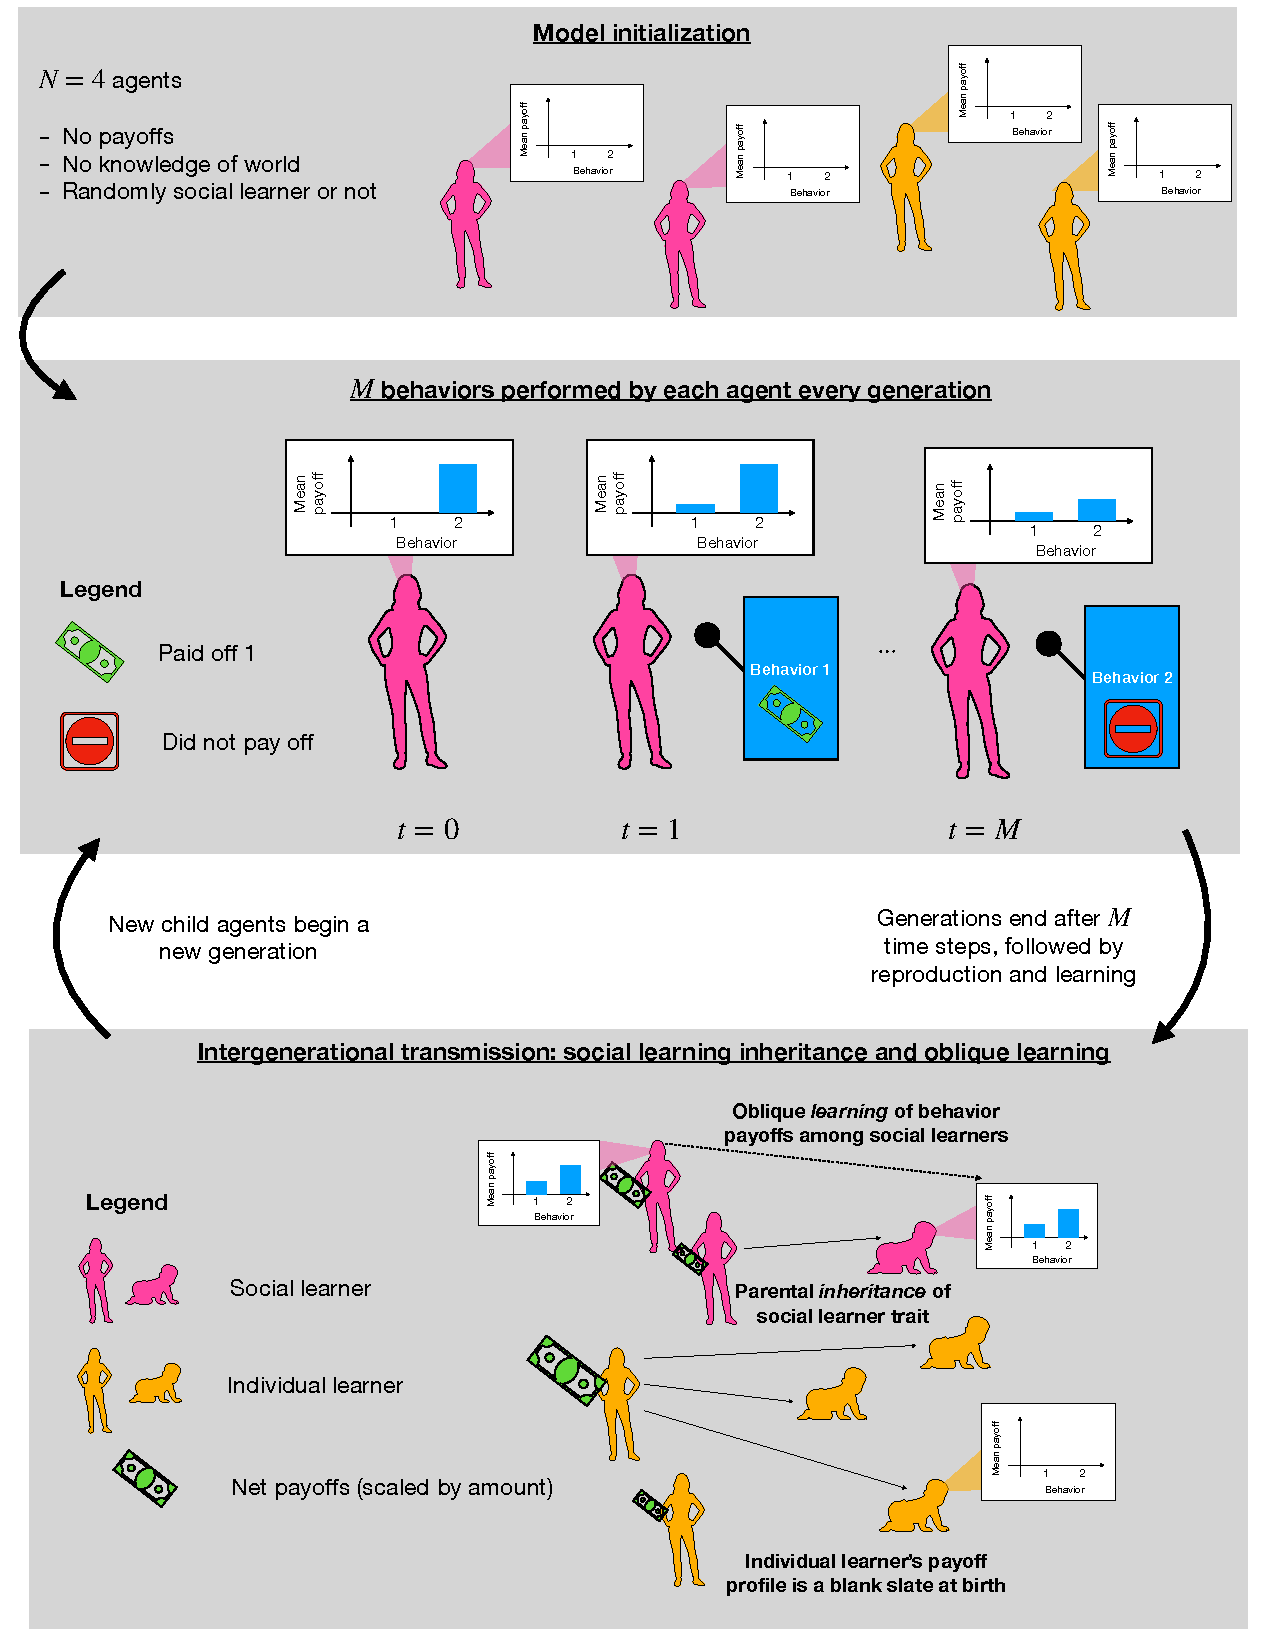
\includegraphics[width=\textwidth]{Figures/IntraInterGenerationalDynamics.pdf}
\end{figure}


We identified four ``principal components'' of uncertainty that affect the
ability of agents to find and choose the optimal behavior: 
\emph{environmental variability}; \emph{payoff ambiguity}; \emph{selection set size}
(number of behaviors environment affords); and the \emph{effective lifespan}.
Environmental variability, denoted $u$, is the probability that the behavior
yielding the optimal payoff, $\pihigh$, changes from one generation to the next.
We operationalized payoff ambiguity by setting $\pihigh = 0.9$ for all analyses
and varying $\pilow \in \{0.1, 0.45, 0.8\}$. The selection set size is the
total number of possible behaviors agents choose from, denoted $B$. The 
effective life span is the number of time steps agents live for, which is
also the number of behaviors each agent performs each generation.

\vspace{2em}
\begin{table}[h]
    \caption{Global environmental and cognitive initialization parameters.
      Bold indicates \emph{default value tested}.
    \mt{TODO: Test more $N_\text{T}$ for sensitivity analysis}}
    \label{tab:modelParameters}
    \centering %\hspace{-3em}
    \begin{tabular}{cp{4.0in}p{1.25in}} \toprule

        Symbol & Description & Values tested \\ 

        \midrule  

        $B$       & Number of possible behaviors (represented by ``bandits'') 
                  & 2, 4, 10 \\

        $\pihigh$ & Probability that the unique optimal behavior pays off 1 
                & \textbf{0.9} \\

        $\pilow$ & Probability one of $B - 1$ non-optimal behaviors pays off 1 
                 & 0.1, 0.45, 0.8 \\ 

        $\tau$ & Softmax temp.; $\uparrow=$more exploration, $\downarrow=$more
                    exploitation 
               & 0.01, \textbf{0.1}, 1.0 \\
        
        $u$    & Probability optimal behavior changes between generations 
               & 0.0, 0.1, \ldots, 1.0 \\

        $L$    & Number of time steps per generation & 1, $B/2$, $B$, $2B$, $4B$ \\

        $N_T$    & Number of teachers to pool, from which best selected 
                 & \textbf{5}  \\

            
               
        \bottomrule
        \end{tabular} 
\end{table}


To guide behavior selection, agent $i$ counts how many times it
performed each behavior $b$, denoted $c_{ib}$. Agents use this count to 
update the mean payoff they have obtained from behavior $b$, denoted $\ledger$.
$\ledger$ is initialized to 0 for all $b$ at model start for
all agents (Figure~\ref{fig:schematic}A), and at 
generation start for asocial learners. Social
learning agents' $\ledger$ is initialized as that of its teacher, who is selected
through performance-biased oblique learning; $c_ib$ is set to 1 for all social
learners $i$ and behaviors $b$ (Figure~\ref{fig:schematic}C). Agent $i$'s
accumulated payoffs from performing several behaviors over their lifetime of $L$
time steps is denoted $\pi_{i}$. If an agent $i$ is a social learner, then we write
$s_i = 1$, otherwise the agent is an asocial learner and $s_i = 0$.

At generation start, one of the behaviors is set to 
yield expected payoff $\pihigh$, with the other $B-1$ behaviors yielding
expected payoffs $\pilow$. At each time step, agents perform behavior $b$ 
with softmax-weighted probability
\begin{equation}
  \Pr(\text{Agent $i$ performs behavior $b$}) = 
    \frac{e^{\beta \ledger}}{\sum_{b=1}^B e^{\beta \ledger}},
\end{equation}
\noindent
where $\beta$ is a parameter that adjusts how frequently agents perform 
behaviors with high expected payoffs (larger $\beta$) versus how frequently
agents explore alternative behaviors (smaller $\beta$)~\cite{McElreath2005}. 
Agents probabilistically recieve a payoff of 0 or 1 depending on whether the
bandit paid off, equivalent to a draw from a Bernoulli distribution with 
mean $\pi_b$. For concreteness we denote this probabilistic payoff
$\bandit$. On performing behavior $b$, agent $i$ updates the
corresponding behavior count by 1, $c_{ib} \leftarrow c_{ib} + 1$, and then
the expected payoffs calculated for that behavior are updated with
exponentially-weighted averaging
\begin{equation}
  \ledger \leftarrow \ledger + \frac{\bandit - \ledger}{c_{ib}}.
\end{equation}
\noindent
This procedure continues for $L$ time steps within each generation
(Figure~\ref{fig:schematic}B).

In between generations agents first reproduce via asexual haploid reproduction; 
then new child agents learn from the
previous generation if they are social learners; and finally all agents from the
previous generation then die off (Figure~\ref{fig:schematic}C). 
$N$ reproducers are selected with replacement over $N$ independent draws, 
biased by performance:
\begin{equation}
  \Pr(\text{Agent $i$ is chosen to reproduce in one draw}) = \frac{\pi_i}{\sum_{i=1}^N \pi_i}.
\end{equation}
\noindent
A child inherits its parent's social learning trait $s_i$ without mutation.
A social learner child with $s_i = 1$ learns from a teacher from its parent's
generation, including possibly their parent (oblique learning). 
A child selects its teacher by first selecting $N_T$ prospective
teachers from the population completely at random, then selecting the one with
highest net payoffs $\pi_i$ as their teacher, with ties broken randomly ($N_T =
5$ in the main text; \mt{Other values will be tested in the supplement}). While it
is somewhat arbitrary to first subset $N_T$, this is a conservative choice that
represnts the fact that access to the entire population is not generally guaranteed.
Social learners adopt their chosen teacher's ledger of expected payoffs $\ledger$,
and set all $c_{ib} = 1$ so expected payoffs remain within $[0, 1]$.  Asocial
learners ($s_i = 0$) are initialized with all $c_{ib} = 0$ and $\ledger = 0$ 
(Figure~\ref{fig:schematic}C). The
newly initialized population then begins behavior selection and payoff accumulation
for another $L$ time steps. The evolutionary process continues until $\sum_i s_i
= 1$ or $\sum_i s_i = 0$ \mt{I believe all trials will eventually end like this, so
in the next set of model runs I will not allow early termination before one of these
conditions are met}.

\begin{table}[h]
    \caption{Outcome variables.}
    \label{tab:outcomeVariables}
    \centering %\hspace{-3em}
    \begin{tabular}{cp{4.25in}p{0.85in}} \toprule

        Symbol & Description & Values \\ 

        \midrule  

        $\meansl$ & Mean social learning prevalence over agents and trials
                  & $\in [0.0, 1.0]$ \\

        $\meanpi / L$ & Mean payoffs accumulated in a generation normalized by
        lifespan & $\in [0.0, 1.0]$ \\

        $\meanT / L$ & Mean number of generations to convergence & 20k / 8 max. \\
        \bottomrule
    \end{tabular}
\end{table}

To analyze the effect of the four principal uncertainty factors, we systematically
varied their values and observed three key outcome variables aggregated across 1000
trial simulations, and across all agents when appropriate. We varied $u \in \{0.0,
0.1, \ldots, 1.0\}$; $\pilow \in \{0.1, 0.45, 0.8\}$; $B \in \{2, 4, 10\}$; and $L
\in \{1,2,4,8\}$ for $B=2$ and $L \in \{1,B/2,B,2B\}$ for $B=4,10$.  We observed
three outcome measures: (1) $\meansl$, the average value of $s_i$ over all agents
and trials; (2) $\meanpi / L$, the average net payoffs at simulation end across
agents and trials, normalized by lifespan; and (3) $\meanT / L$, 
or the mean number of time steps to fixation normalized by
lifespan\footnote{Equivalent to the mean number of generations to fixation}
(fixation means $\sum_i s_i = 0 \text{ or } 1$). \mt{Make sure to qualitatively
introduce these and their evolutionary importance in the intro.}
We analyze outcomes by plotting $\meansl$ on the y-axis and environmental
variation is on x-axis since we theoretically expect that $\meansl$ will 
decrease monotonically from 1 to 0 as $u$ increases. We expected and observed
that the other three uncertainty factors shift the value of $u$ at which 
$\meansl$ starts to decrease, and how rapidly $\meansl$ decreases. Note that the
hypothesis-testing concept of significance is meaningless here because we could
make any small outcome difference ``significant'' by running more simulation trials.
We instead study the patterns of outcome 
variables over systematically varied uncertainty factor values. 
Our model was implemented in the Julia programming language~\cite{Bezanson2017} 
using the Agents.jl agent-based modeling library~\cite{Datseris2022} and run
on the Sherlock supercomputing cluster at Stanford University. Model code and
data are publicly available on GitHub\footnote{\url{https://github.com/mt-digital/UncMod}} 
and OSF.io\footnote{\mt{TODO}}.


\section{Analysis}

Several patterns emerged in changes to the shape of social learning suppression over
environmental variability, $u$, across different uncertainty contexts defined by the
payoff ambiguity, selection set size, and effective lifespan
(Figure~\ref{fig:mainResults}). When payoff ambiguity and selection set size were
both small ($\pilow = 0.1$ and $B=2$) social learning only evolved when $u$ is small
since individual learning is relatively efficient in this case
(Figure~\ref{fig:mainResults}, upper left). As $\pilow$ increased the suppression of
$\meansl$ flattened over $u$, which was more pronounced for smaller $L$ (rows of
Figure~\ref{fig:mainResults}).  When $L$ is smaller, agents have fewer opportunities
to learn through trial and error, and so it is more difficult for them to discern
which strategy, social or asocial, is optimal. Increased selection set size led to
both a shift in the critical value of $u$ when $\meansl$ begins to decrease, and
flattened social learning suppression. This is because possibly misleading 
social information is less consequential due
to (1) larger $B$ is a more difficult problem for trial-and-error learning, and
(2) a misidentified optimal behavior is weighted less relative to smaller
$B$, meaning agents are more likely to explore behaviors identified as non-optimal
when $B$ is larger (columns of Figure~\ref{fig:mainResults}).  \mt{Support this by calculating the difference between weights when B=2 and B=10 and a social learner learns outdated information}
Increased $B$ led to more pronounced flattening of social learning suppression when
$L$ was small, apparently again because of the limited data available to evolution,
making individual outcomes more path dependent.

\begin{figure}
  \caption{Social learning prevalence (y-axes) monotonically decreases as 
  environmental variabilty, $u$, increases (x-axes) in most uncertainty contexts. 
  Other uncertainty values $\pilow$ (rows), $B$ (columns), and $L$ (keys)
  shift and flatten the decrease from all-social-learner populations to all-asocial 
  populations.}
  \label{fig:mainResults}
  \centering
    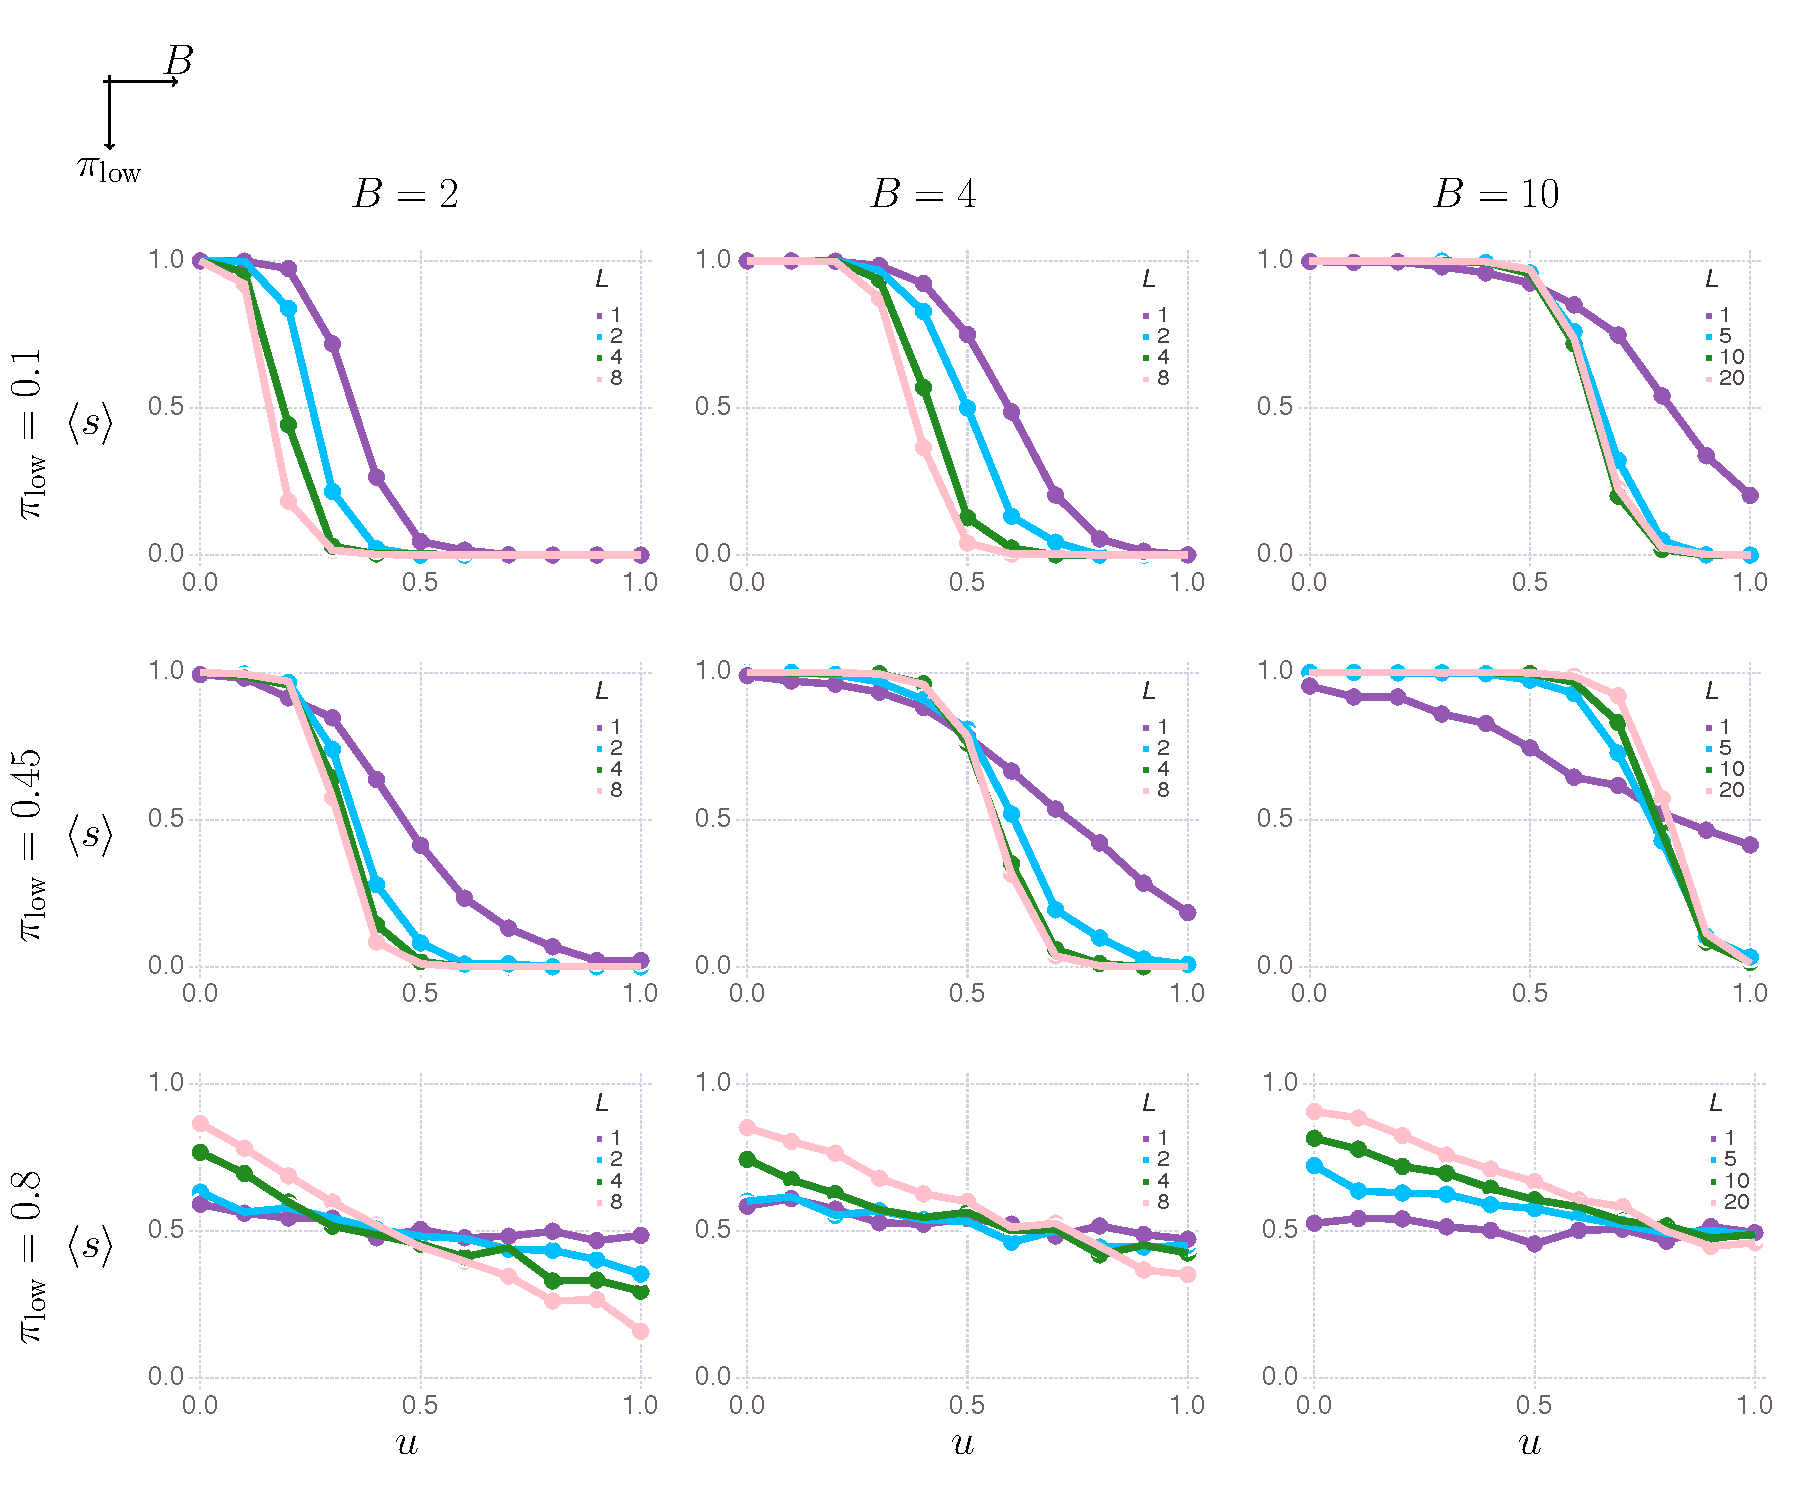
\includegraphics[width=\textwidth]{Figures/mainResultsPlots.pdf}
\end{figure}

Social learning evolution was correlated with differences in population-level
expected payoffs for social versus asocial learning. Furthermore, we found that mean
payoffs realized by our simulated agents track either the expected social learning
payoffs, $\meansoc$, or the expected asocial learning payoffs, $\meanasoc$.
$\meansoc$ and $\meanasoc$ were calculated across uncertainty contexts by
initializing the model to be all social or all individual learners then running the
model for 100 generations for social learning and across 1000 one-generation trials
for individual learning.  Simulated evolutionary mean payoffs across agents and
trials, $\meanpi$, are initially higher than expected asocial learning, $\meanasoc$,
and comparable to expected social learning, $\meansoc$, in most cases 
(Figure~\ref{fig:payoffs}).  But as social learning becomes less beneficial due to
increased environmental variability, $\meansoc$ and $\meanpi$ approach $\meanasoc$.
It appears agents tend
to be conservative as expected social and asocial learning payoffs approach each
other---the transition to $\meansl = 0$ often happens although social
learning is still theoretically optimal. When $L=1$, $\meanpi$ can be greater than
$\meansoc$ because asocial learners at the beginning of the simulation help to 
pass on less misleading information on average, so that the cultural information passed on by
eventual all-social learner populations have more noise. This noise further reduces the
weighting of the previous generation's observed optimal payoff if it changes between
generations enabling agents to more efficiently explore alternatives before focusing
on a misidentified optimal behavior \mt{I think we could calculate this if it were
valuable}. 

\begin{figure}
  \caption{Mean payoff normalized for lifespan (y-axes, solid lines with circles)
    generally track either expected all-social-learners payoff ($\meansoc$, dash-dot
    line with diamonds) or expected all-asocial payoff ($\meanasoc$, long dash
    horizontal lines) as $u$ increases (x-axes). When $\meansl$ goes from 1 to
  0 is when social learning payoffs approach individual learning payoffs due to
increased environmental variability.} 
  \label{fig:payoffs}
\centering
    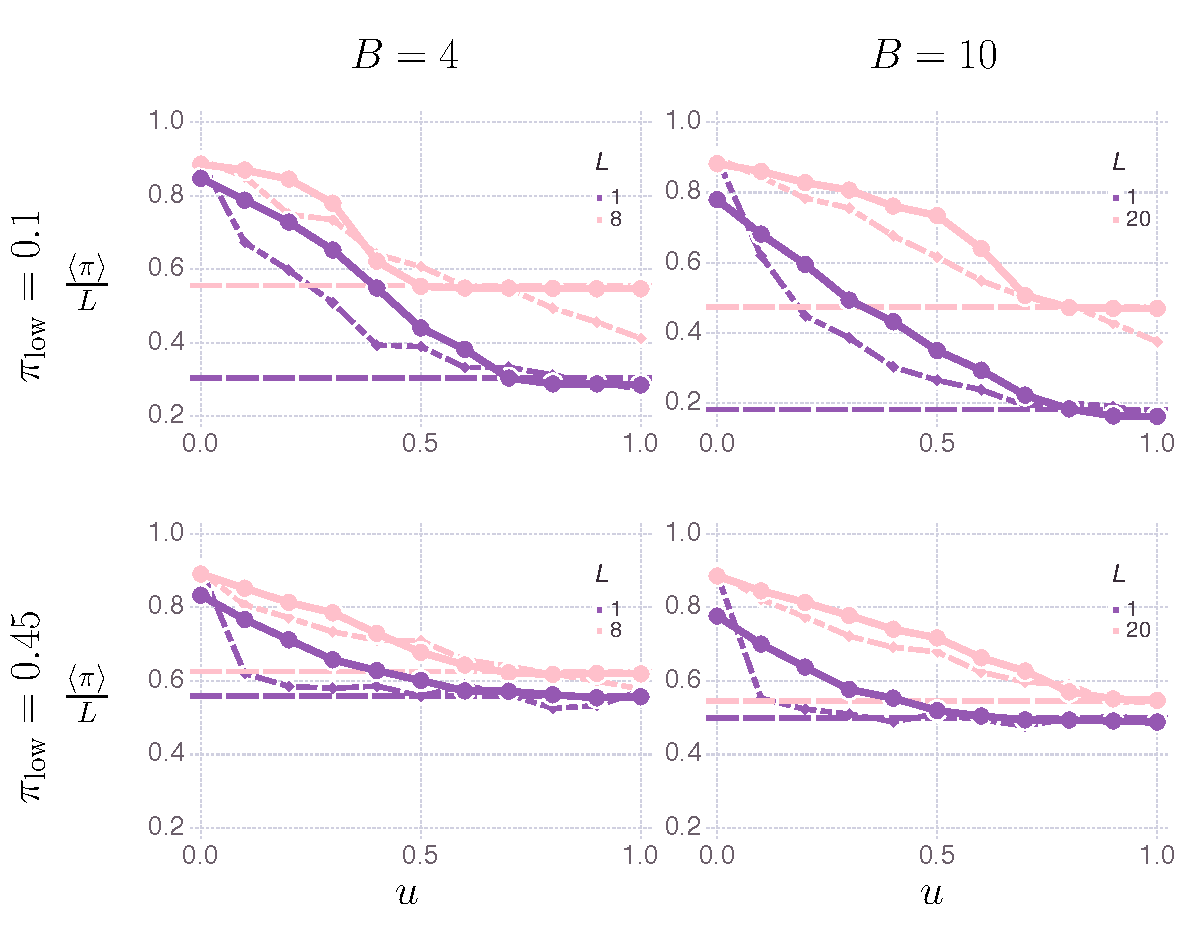
\includegraphics[width=0.75\textwidth]{Figures/meanNetPayoffs.pdf}
\end{figure}

The number of generations to reach fixation increased
when expected social learning payoffs approached expected asocial payoffs, i.e.,
when $\meansl$ becomes suppressed (Figure~\ref{fig:steps}). Recall a fixated
state is when $\sum_i s_i = 0 \text{ or } 1$.  This supports our explanation that
the supression of social learning begins when individual simulation outcomes are
more path dependent and susceptible to end in a non-optimal state since simulations
in these conditions also take longer to reach fixation.  For example, when
$\pilow=0.1$, $B=4$, and $L=8$, we see a sharp increase in $\meanT$ when social learning
suppression begins; but when $L=1$, social learning suppression is flatter
than for $L=8$, and  correspondingly its $\meanT$ is not as strongly peaked, but is
elevated across the $u$ (Figure~\ref{fig:steps} upper left).  In some cases $L=1$
trials reached fixation faster than $L=8$ or $L=20$; larger $L$ had larger peak $\meanT/L$
than smaller $L$, for example, both for the cases shown in Figure~\ref{fig:steps}
and across all settings tested \mt{TODO: add full figure to SI}. 
However, we also see situations where $L=1$ and fixation takes longer than $L=8$.
This is especially pronounced for
$\pilow = 0.45$ where social learning suppression is much flatter for $L=1$
(Figure~\ref{fig:steps}, bottom row). In general, then, a sharper peak in $\meanT$
indicates a sharper suppression of social learning over $u$ and a flatter peak,
elevated over more values of $u$, indicates greater path dependence and more 
drift overall.


\begin{figure}
  \caption{Average number of generations ($\meanT/L$, y-axes) for populations to fixate
  where agents either all become social or all become asocial learners. As
  $u$ increases (x-axes) models take longer to fixate due to drift, up to a point,
but then fixation accelerates as individual learning becomes more obviously 
superior. Increased $\pilow$ increases time to fixate; both $\pilow$ and $B$
shift peak time to fixation over $u$.} 
  \label{fig:steps}
\centering
    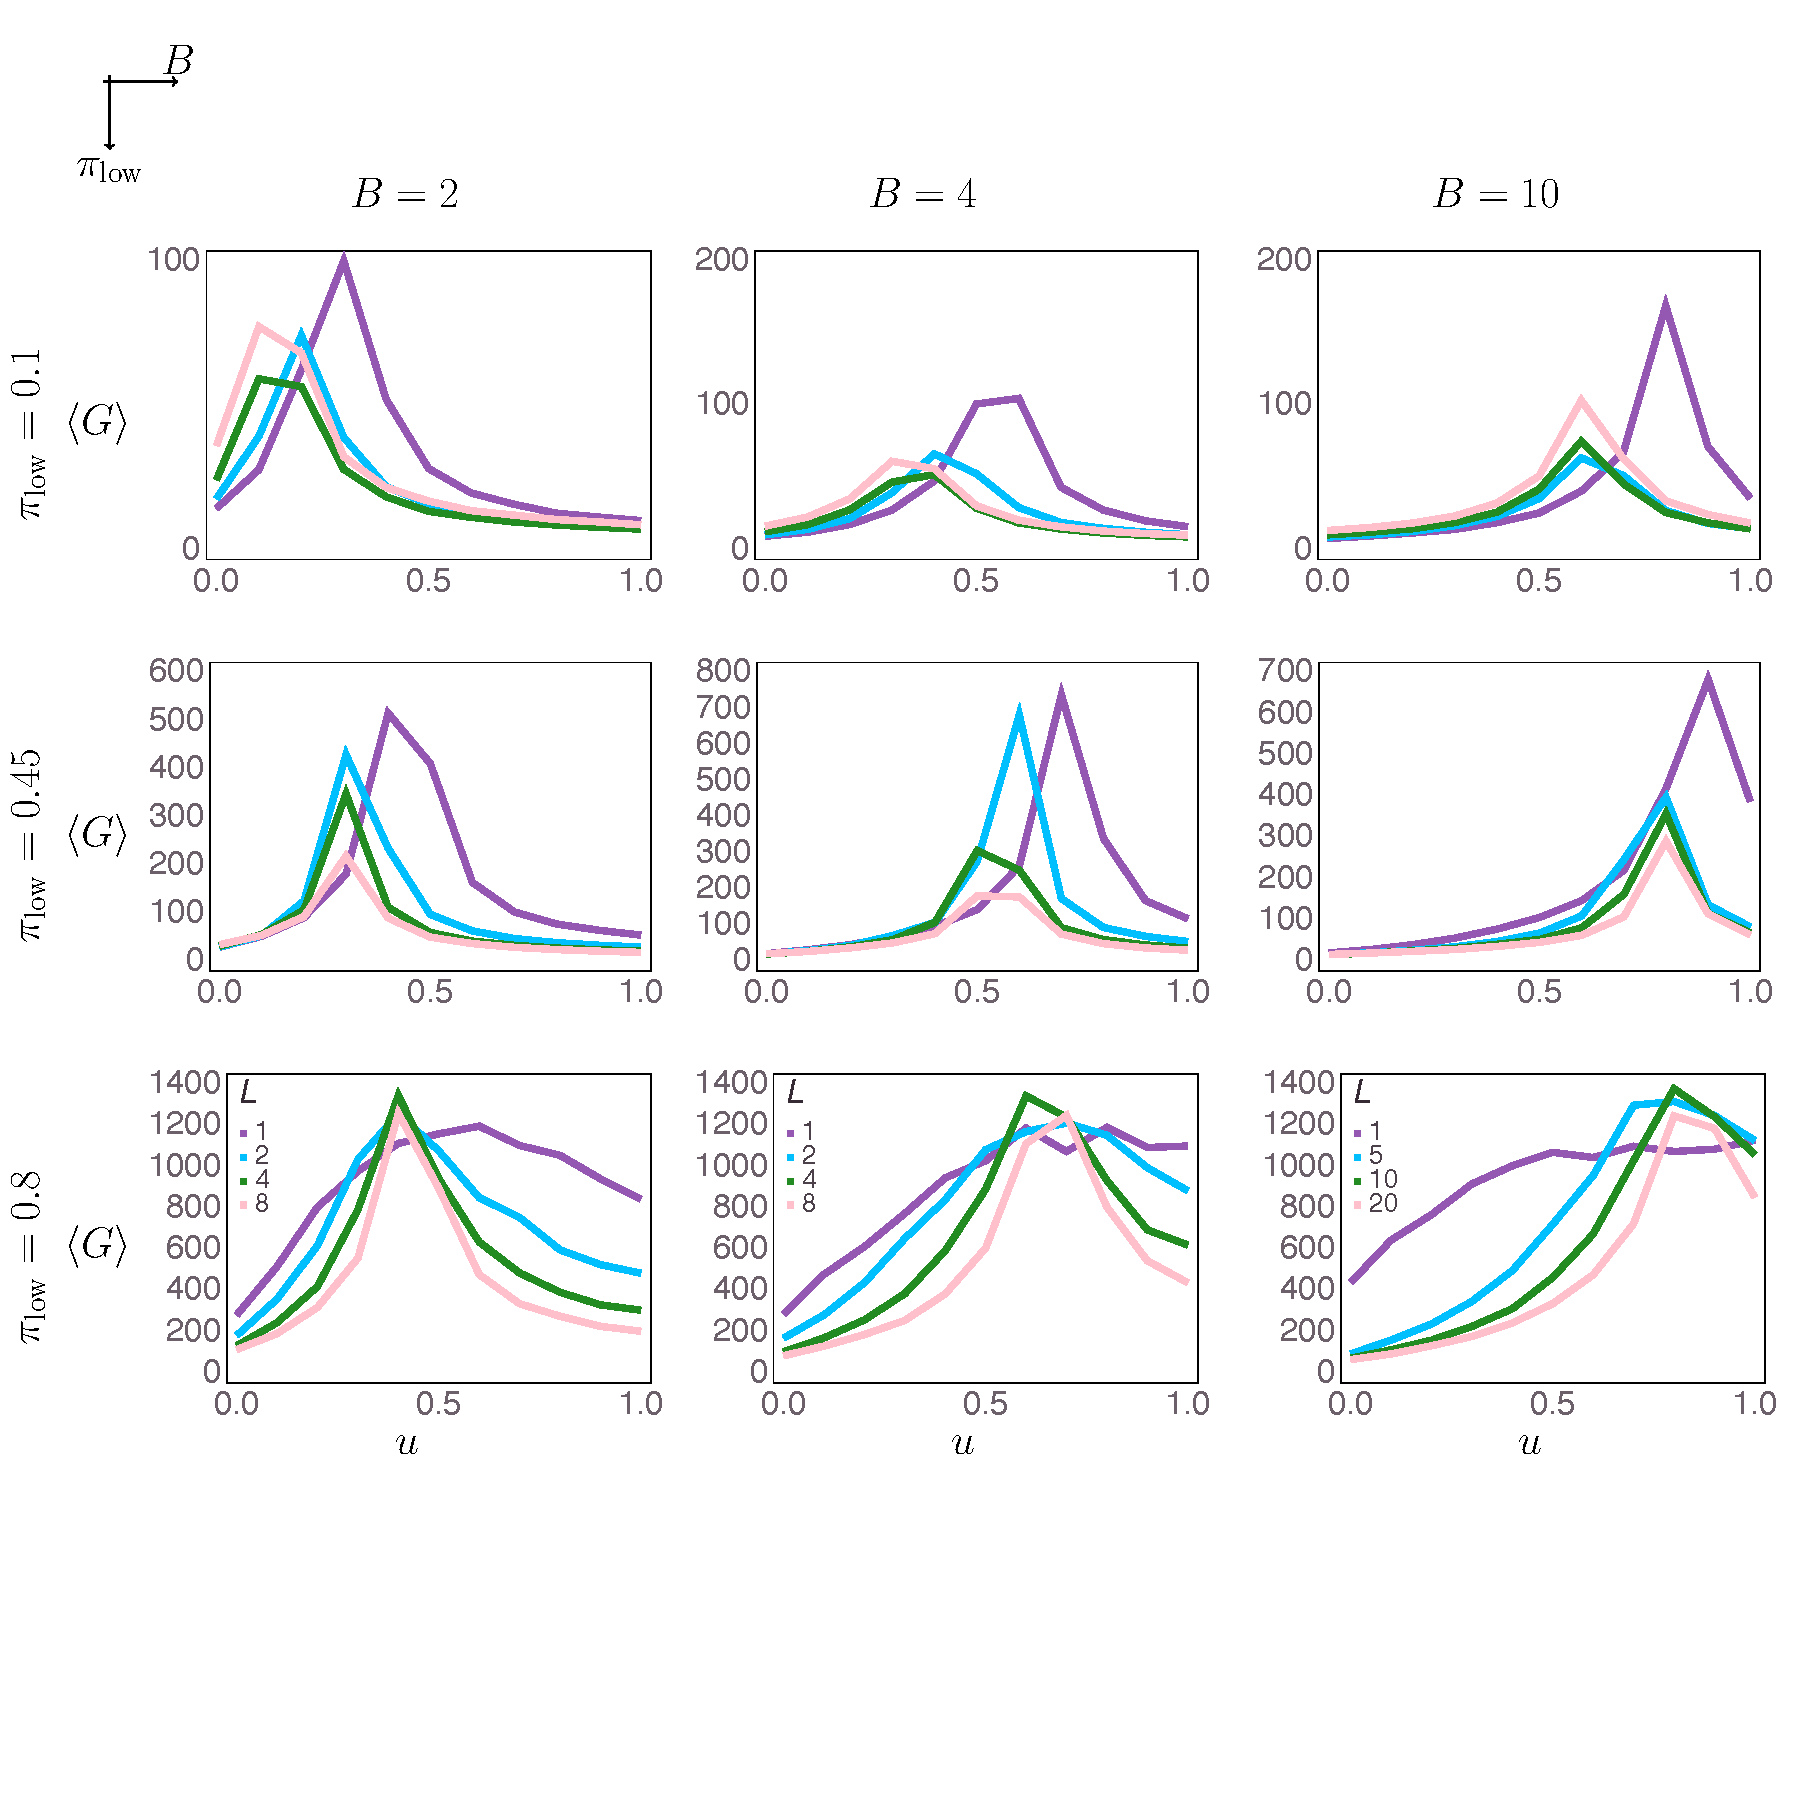
\includegraphics[width=0.75\textwidth]{Figures/stepResultsPlots.pdf}
\end{figure}

\section{Discussion}

By identifying four common uncertainty dimensions we developed a model that predicts
how different forms of uncertainty might interact to foster or suppress social
learning.  The model reproduced classic predictions that social learning can yield
higher payoffs than individual learning when uncertainty is sufficiently limited.
By disambiguating and organizing various operationalizations of uncertainty, 
we developed a more nuanced theoretical understanding of which forms of
uncertainty interact in which ways to make social learning more or less beneficial
compared to asocial learning.  Note that in many cases we made modeling choices that
excluded some important mechanisms of social learning; for example we assumed
success-biased learning, although conformity is theoretically important as
well~\cite{Muthukrishna2016a,Smaldino2018b}. Still, we believe our model
advances theoretical parsimony; and the software implementation is designed to
facilitate testing alternate modeling choices. 

\paragraph{Disc. 2: Foundation for studying social learning evolution with group
structure or other topics(PAUL, JAMIE, CRISTINA)}~\cite{Katsnelson2014}.

Our modeling approach may have applications to developing social artificial
intelligence. Much effort has gone in to developing the cognitive machinery to
realize multi-agent reinforcement learning
systems~\cite{Sandholm1996,Ndousse2021,Gronauer2022}, with some work explicitly
incorporating cultural evolutionary approaches to social learning~\cite{Jaques2019}.
However, it seems there are a lack of methods for adapting to environmental
uncertainty, or determining when social learning is actually advantageous under
different uncertainty conditions. Our model dynamics could be used as an
evolutionary algorithm to update AI agents' social learning strategy without
explicit knowledge of, or need to approximate, the underlying uncertainty structure.
Our model could also predict the expected benefit of social learning, which may be
inherently costly in artificial multi-agent learning systems, and how long the
translated evolutionary algorithm may take to converge.



\bibliographystyle{apacite}
% \bibliography{/Users/mt/workspace/Writing/library.bib}
\bibliography{this.bib}

\appendix


\section{Appendix}

\subsection{Convergence information}

\begin{table}[h]
  \caption{Max. iterations = 5000.}
  \label{tab:convergence}
  \centering
  \begin{tabular}{cccc} \toprule
    $B$ & \# not at fixation & \# total series & Pct. not fixated \\
    \midrule  
    2  & 0  & 132000 & 0.0 \% \\
    4  & 0  & 132000 & 0.0 \% \\
    10 & 44 & 132000 & 0.00033  \% \\
    \bottomrule
  \end{tabular} 
\end{table}

\end{document}
